%\section{DOFs}

\section{DoF/FEM Module}
\label{sec:dof_module}

In the context of the finite element method solutions are expressed in terms of linear
combinations of some chosen shape functions defined on mesh cells. 
The degrees of freedom (DoF) represent the finite
number of parameters that define such a discrete function. The number
of DoFs can easily count up for millions of unknowns and can typically
be associated with locations which are distributed over the mesh.
In the following, the DoF/FEM module will be 
described, representing the finite element ansatz (submodule FEM) 
and the challenging treatment of the degrees of freedom (submodule DoF).

\subsection{FEM Submodule}

This submodule is dedicated to represent a finite element ansatz in a
generic way to ensure extensibility at low memory costs, but still
to enable high performance assembly. The basic concept lies in defining
three major classes \code{FEType}, \code{FEManager} and \code{FEInstance}.
The first one, \code{FEType}, is an interface class and deals with 
representing a specific continuous or discontinuous finite element 
ansatz on a defined reference cell. For instance a Lagrangian
element \code{FELagrange:FEType} is a specialized implementation
and defines the necessary parameters, such as the polynomial degree. 
Also, since each ansatz has a specific number of degrees
of freedom, these are initially defined on this cell and stored
in a lexicographically order (see figure \ref{fig:Lexicographic-numbering}). 
\begin{figure}
\noindent
\begin{centering}
\includegraphics[height=2.8cm]{fig/dof7}
\par\end{centering}
\caption{\label{fig:Lexicographic-numbering}Lexicographical numbering of the DoFs on the reference cell.}
\end{figure}
Further, interfaces to compute the values of the shape functions, which indices 
correspond to the local cell numbering, etc. are provided. 
To add a new finite element ansatz, a new class needs to be derived from 
\code{FEType} and the few needed functions must be implemented. It is
guaranteed that the new elements can be used all over the library, which
makes extensibility easy. 
\par 
On every mesh cell and for every variable a specific finite element
ansatz is prescribed. Therefore, a design pattern from software engineering
known as "singleton" is implemented, which means that every ansatz which occurs
more than once is represented and stored in only one element, managed 
by \code{FEInstance}. For establishing the mapping between a tuple
of a mesh cell and a variable to their corresponding singleton, only \emph{references}
are stored. This mapping and all interfaces to out-of-module classes are
managed by the \code{FEManager}. Especially, each mesh cell has a mapping
from physical space to the reference cell, depending on its geometry and finite
element ansatz, which is also stored within \code{FEManager}. To give an example, 
for Lagrangian elements on hexahedrons, this results in a trilinear transformation. 
Since for a new ansatz a new mapping is needed, it also can be implemented as a 
derived class from \code{CellTransformation}.
\par 
This separation of tasks leads to a generic and efficient way of representing
a finite element ansatz. At this stage of HiFlow$^3$ not only arbitrary degrees 
of Lagrangian elements can be incorporated, but also their usage in an assembly 
routine is with high performance, since each shape function can be evaluated
and stored for each singleton and therefore does not need to be computed on the fly.


\subsection{DoF Submodule}

Considering as an example typical fluid problems in three dimensions, one needs to deal
with a finite element ansatz for four scalar variables (three velocities and one pressure).
For a complex unstructured geometry, this easily can lead to a very high number 
of unknowns ($\gg$ 10.000.000) alias degrees of freedom. These DoFs need to be
numbered and interpolated in an unique way depending on arbitrary combinations
of finite element ansatz on neighboring cells. For a continuous ansatz, given 
the local numbering strategy provided by the submodule FEM on each cell, one major 
task is to create a mapping between a local DoF Id and a global (mesh wide) DoF Id. 
The second major task is to interpolate those DoFs, which are restricted due to
conditions provided by FEM and cannot be identified. Such cases can occur for example
in the case of h-refinements (hanging nodes), p-refinements or hp-refinements
(see figure \ref{fig:Degrees-of-freedom}).  

\begin{figure}
\noindent
\begin{centering}
\includegraphics[height=2.8cm]{fig/dof1a}
\includegraphics[height=2.8cm]{fig/dof1b}
\includegraphics[height=2.8cm]{fig/dof1c}
\par\end{centering}
\caption{\label{fig:Degrees-of-freedom}Degrees of freedom in h-refined (left), p-refined (middle) and hp-refined (right) setting. Green marked DoFs are interpolated due to continuity constrains.}
\end{figure}

As mentioned in the previous subsection, the DoFs in any cell of the
considered mesh are determined by a transformation that maps the
reference cell to the chosen physical cell and thereby defines the
location of the DoF points (see figure
\ref{fig:Transforming-DoF-points}).  At that state the DoF Ids can be
defined and numbered consecutively in the order of a given iteration
through the mesh cells and the local FEM numeration scheme. Further a
mapping that maps a cell index of the mesh and a local DoF index (key)
to the corresponding DoF Id (value) is created. This is done for each
variable of the underlying problem. If no continuity constraints are 
set for the global DoF numbering procedure, the resulting numeration is 
appropriate for discontinuous finite element methods.
\par
In case of constraints (i.e. continuity constraints) an interface 
approach is realized for the calculation of the interpolation and 
identification of DoFs on neighboring cells. In
this context \emph{interface} denotes the common cell boundary between
two neighboring cells. By this, it is possible to handle all types
of neighboring finite elements in a generic way, and as expensive
local calculations are made only once for each occurring type of interface,
the overall performance is still very good. Through an iteration over all 
interfaces of the mesh, a so-called \emph{interface pattern} is determined that includes the
geometrical information (orientation of cells, h-refinement status,
etc.) as well as the finite element ansatz of the participating cells
such that all information needed to characterize the interface is
included. With the information contained in the pattern the corresponding
DoF interpolation and identification in terms of the local DoFs are
calculated. Therefore the general transfer operator of Schieweck \cite{Schieweck}
is used that allows interpolation between different finite element
spaces. An important step within this phase is the transformation
of DoFs of a neighboring cell next to the reference cell (see figure
\ref{fig:Transforming-DoF-points}). Once this local evaluation is
done, the tuple of the pattern description (key) and the interpolation
and identification information (value) are stored in a map structure
that allows for fast access given a pattern description. Using this
map the interpolation and identification of DoF Ids can be realized
efficiently even in the complex hp-refined context using an equivalence
class generator. Later on the numbering of the
DoF Ids can be changed easily by applying some user defined permutation.


%
\begin{figure}
\noindent \begin{centering}
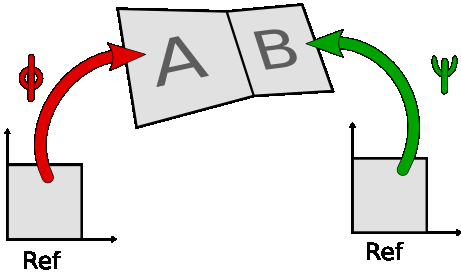
\includegraphics[height=3.4cm]{fig/dof3}\hfill{}\hfill{}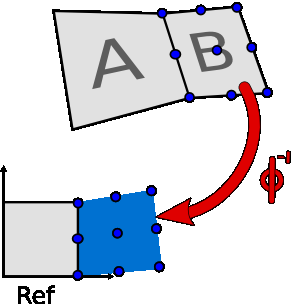
\includegraphics[height=3.4cm]{fig/dof5}
\par\end{centering}

\caption{\label{fig:Transforming-DoF-points}Transformation of DoF points to a cell
in mesh (left). Transformation of DoFs of neighboring cell next to the reference cell (right).}

\end{figure}

\subsection{Partitioning}

In a domain decomposition setup, i.e. several processes are used for
the solution of one single domain, each part of the domain (subdomain)
is dedicated to one process using MPI. Again a unique DoF numeration
of all DoFs in the global domain must be determined. For good scaling
properties, a parallel and distributed handling of the DoFs is needed,
i.e. each process manages the DoFs that are connected to the cells
lying in its domain and the class \code{DofPartition} is used to create
the correspondence with other subdomains from other processors via
MPI communication. Each subdomain has information of the neighboring
domains by the \emph{ghost cells} (one \emph{ghost layer}), which
are represented by the red cells in figure \ref{fig:Two-domains-with}.
To create a DoF numbering with (domain-) global Ids, each process determines
in a first step a consecutive numbering of the DoFs within its subdomain,
whereas also the ghost layer is treated as if it would belong to the
subdomain. Next, the antiquated information stored in this layer needs
to be updated via communication. Hereby, a decision needs to be made,
whether a DoF lying on the skeleton of the domain belongs to a subdomain
or not, i.e. this DoF is lying on two subdomains, which are sharing
it. The implemented procedure states, that the subdomain represented
by a unique lower subdomain Id will own the DoF. Hence, identification
and interpolation is possible. At the final stage,
every subdomain has a unique numbering, containing the correct DoF
Ids in its ghost layer.
\begin{figure}
  \centering
  \includegraphics[height=4cm]{fig/dof6}
  \caption{\label{fig:Two-domains-with}Two domains with ghost cells}
\end{figure}
